% CHAPTER 3 LESSON 2
\clearpage
\section{Digitization of speech signals (time-amplitude)}
\label{Digitization of speech signals (time-amplitude)}

Spectral transformation, digitation of speech and audio signla.s This is what we are really aiming for. So what we would have is a microphone somewher in the room and now we speak into the microphone and eventually what you would do if you would like ti store the signal on a diital device or would like to transmit it through a digital channel  for instance a cell phone, we would firat need to digitalize the signal which involves a discretization of the time axis, so how is this done .

First of all if you have a signal and you would like to discretize it. It basically means that you take snaphots a certain unstances in time  and when you look at such a signal, it basically means that you dont really know what goes on inbetween two samples.  Then, the sampling theorem tellls you that if you have a sample rate that is high enough, you can still perfectly reconstruct you signal. Of copurse in sampling, you would like to use as few samples as possible because if you have too many sampling points, that would e a redundancy and that would be a waste of data storage, if you wanted to sotre the signal on a computer, or if you wanted to transmit the signal then the data rate that we would need would be too high. SO we want the sampling frequency to be as low as possible.And theit is important to understand how low you can go.

Sampling:

If you discretize a signal, you can think of it as the multiplecation of signal with a delta comb or an impulse train.  Now we want to understand what goes on in the frequency domain. We can use the property that the multiplecation in time domain corresponds to convolution in frequency domain. Because then,m if you know this you can compute the spectrum of the original signals, and loko at the result. And from this we can derive the necessary conditions that we need to fulfill in order to reconstruct our signal perfectly..

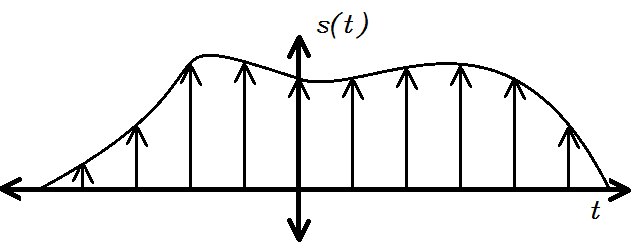
\includegraphics[width=0.5\linewidth]{Pictures/Chapter_2_Lesson_1/Sampling4.png}

So lets assume that we obtain our discrete signal by multiplying our signal with an impulse train:

\begin{equation*}\discFunc(\sampTime) = \contFunc(\sampTime)\cdot\Sh(\frac{\sampTime} {\samplingPeriod})\text{          with \begin{math}\samplingPeriod = \frac{1}{\samplingFreq}\end{math} the sampling period }\end{equation*}

The impulse train is given as a series of delta pulses spaced at Ts:

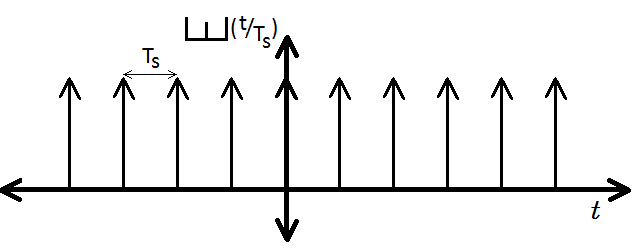
\includegraphics[width=0.5\linewidth]{Pictures/Chapter_2_Lesson_1/Sampling1.png}

So this signal is difined as the sum over infinitely many pulses(delta functions). And the are spaced at a distance of Ts and now here we have multiples of Ts and we have infinitley many that extend into positive and negative time domain.
 
 \begin{equation*}\Sh(\frac{\sampTime} {\samplingPeriod}) = \sum_{\sampIndex}\deltaPulse(\sampTime - \sampIndex\samplingPeriod) \end{equation*}
 
 And now we want to compute the spectrum of this signal.  So to do this we compute the integral over the signal multiplied with the complex exponentials which is basically the definition of the FOurire transform.
 
  \begin{equation*}\fourierSym( \Sh(\frac{\sampTime} {\samplingPeriod})) = \int^{\infty}_{-\infty}\sum_{\sampIndex}\deltaPulse(\sampTime - \sampIndex\samplingPeriod)e^{-jwt}dt  \end{equation*}
 
So how can we solve this integral? Well for instnce by using the sifting property.  This basically states taht if you take the integral of some function f(t) times a shifted impulse, and you integrate over all t, its corresponsd to evaluating the fuinction only at the point T.

\boxed{\int f(t)d(t-T)dt = f(t)\text{      ''Sifting Property''} }

But from because sums and integrals are linear terms, we can shift them.  And then what we get is the sum over infintiely many shifted complex exponential functions:

\begin{equation*}= \sum^{\infty}_{\sampIndex=-\infty} e^{-jw\sampIndex\samplingPeriod} \end{equation*}

So now we have this summation over exponential functions over infinitely many n. So what does this result in.  If I have an exponential function and I sum up over infinitely many n, I will get 0.  Unless wTs  = 0 and multiples of 2pi, because the value of the exponential is one and therefore the summation goes to infinity. SO:

\begin{equation*}= \begin{cases}\infty, & w\samplingPeriod = k2\pi, k \in \mathfrak{Z}.\\ 0, & \text{else}\end{cases} \end{equation*}

SO how can we represent this?  This is is function in spectral domain that is zero everywhere but at certain points it goes to infinity. We can mathematically describe this a a shifted delta function in the spectral domain.

\begin{equation*}= \sum^{\infty}_{k=-\infty}  \deltaPulse(w - k2\pi\samplingFreq) \end{equation*}
\begin{equation*}=  \Sh(\frac{f}{\samplingFreq})\end{equation*}

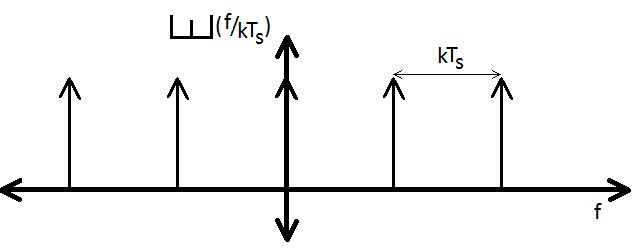
\includegraphics[width=0.5\linewidth]{Pictures/Chapter_2_Lesson_1/Sampling5.png}

So end up with a pulse train in the spectral domain, however the distnace between pusles is no longer the sampling period, but the sampling frequency.  So what have we accomplished here.  We had a continuous time domain signal and we were interested in the resulting spectrum that we obtain when discretize the signal.  We already know that a discrete signal in time domian correpsonds to a periodic signal in frequency domain.  So, but how does it exaclty look and what are the distances between these periodic repetitions, that is something that we just computed cause this distnace will be exaclty the sampling period. SO meaning that in order to compute the spectrum of our signal d(t) what we would need to do is take the fourier transform of our continuous time domain signal x(t) and convoilve it with our impulse response.  Meaning:

\begin{equation*}=\uppercase{\discFunc}(f) = \uppercase{\contFunc}(f)*\Sh(\frac{f}{\samplingFreq}) \end{equation*}

So lets assume X(f) has a certain spectrum something like this:

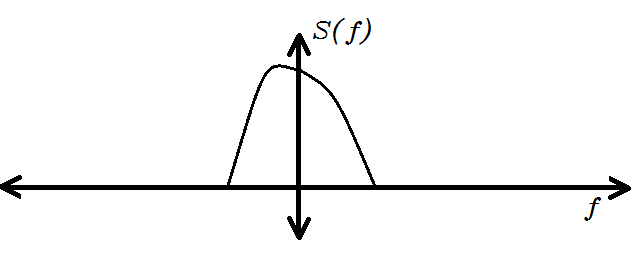
\includegraphics[width=0.5\linewidth]{Pictures/Chapter_2_Lesson_1/Sampling3.png}

and now we convolve this with the fourier transform representaion oif our delta comb

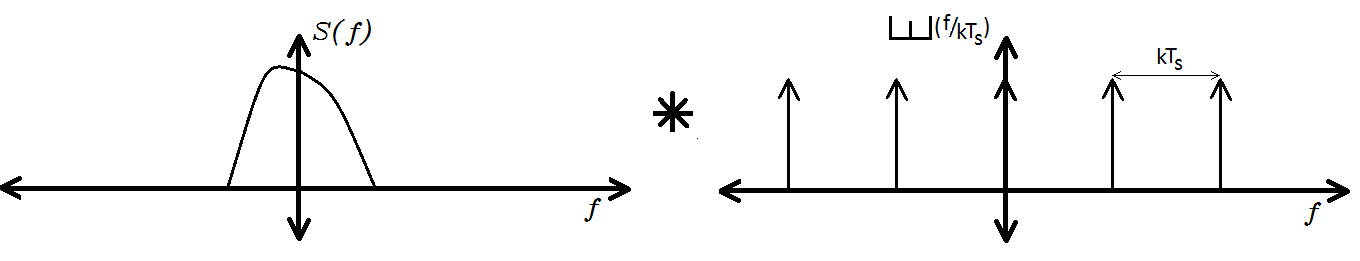
\includegraphics[width=0.5\linewidth]{Pictures/Chapter_2_Lesson_1/Sampling7.png}

SO how would the resulting spectrum look? It would have a periodic representaion.  So what we are drawing here, we can visually derive the sampling theorem.  SO because what happens if we take the sampling frequency too low? If we don not sample our signal often enough.  The replicas of the spectra will overlap meaning that we cannot simply separate the replicas anymore.

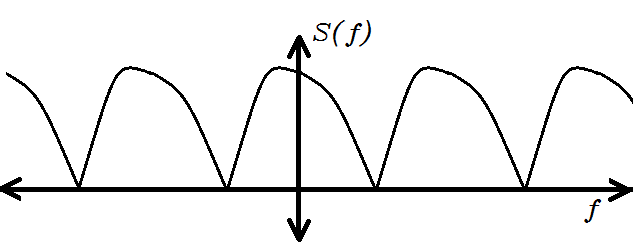
\includegraphics[width=0.5\linewidth]{Pictures/Chapter_2_Lesson_1/Sampling8.png}

SO if fs too low(Ts is too large) then:

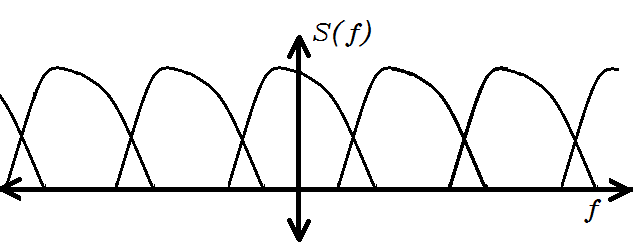
\includegraphics[width=0.5\linewidth]{Pictures/Chapter_2_Lesson_1/Sampling6.png}

 We get our spectrum, except the replicas do not perfectly overlap. This means that we cannot perfectly obtain my signal back again except in trivial examples or specific examples. However, when I have the correctly chosen sampling frequency, then we can simply obtain our signal through lowpass filtering. However this cannot be done when there is an overlap of the signals. SO what does this mean? 
 
 If I choose my smapling frequency, fs, large or equal to 2x's the highest audio frequency, fa. I can perfectly reconstruct the continuous signal x(t) from its discrete representtaion.  
 
 SO this means that if we have a continuous signal, and we sample it with a certain sampling frequency it is true that well you do not sample the samples between two samples. Right so you don not have direct access to these samples, but if the audio bandwidth of this signal is limited it also means that the change between to samples is limited because its a low pass filtered signal in a sense and then if this is the case then you can perfectly interpolate the signal between two samples in a way that you perfectly reconstruct the original continuous signal.
 
 Another way of looking at it or to understand it maybe is that if you have .....what this basically says is that you need a bNDLIMITED SIGNAL that there cannot be a frequency in the signal largeer than fa. that also means that in time domain the change between two samples is limited and so if you fulfill the sampling theorem, you can perfectly reconstruct the signal.
 
 If you obey the Nyquist theorem, tehre is a one to one correspondance between discrete and continuous signals, meaning that we can perfectly reconstruct them.  ANd then if you dont obey it, we get mirror images there will be energy in the signal where it should not be.  If wanted to sample the signal at a lower sample rate, we would need to first apply a low pass.  This would a solution.  Either we could just just a sample frequency high enough, or another thing that we could do if we wanted to choose a lower sample frequency. With speech sounds, we hear these artifacts with high frequency sounds such as s.
 
 SO typical bandwidth that we use.  In telephony, like an ISDN phone but also with your cell phone, we work with sampling rates of about 8khz and then we also low pass filter our signal.  ALthough we have drawn the low pass filter very steep, in practice we cannot realize it this steeply.  So lets say we have speech signals with a bandwidth of up to 16khz.  Then now we use a sampling rate of 8khz, we dont want to havce any information after to 4khz.  But you will not be able to realize low pass filter that has an ideally steep cutoff freequency, but instead, what we would have is something that goes a liitlle more like this... meaning that the spectrum will be distorted up to lower frequencies, and for telephone, the area to where the frequencies are not distorted is 3.4khz. So this is this number here, so theortically speaking, with a sampling frequency of up to 8khz you could recontruct a signal of up to 4khz audio bandwidth, but as you need a vertain lowpass filter that has a certain rolloff the area where the speech is undistorted is only upto 3.4khz.
 
 For music, of course we need higher audio bandwidths,  .....as we said for telephone speech we have 8khz bandwidth, if we have wideband speech telephony, the sampling rate is higher and so the sound quality is better that you can have in a lossless transmission.  Thiese are coding strategies used in some voice over IP clients.  Hifi would be even higher with 44.1kHz, or some standards use 48khz. However at 96khz we are beyond the threshold of hearing and ti makes no sense. 
 
 The next thing that we have to do to discretize a signal, we talked about the discretiaztion on the time axis, but we need to also discrteize the amplitude axis and this.  LATER.
 
 one period no longer fits into one frame  the what happens is, you would basicallc convolve the signal wit ha synch function and you's see samples of the synch function and then you would take discrete samples at theese points.  and then you can imagine that if you have closely spaced sinusoid you will not be able to resiolce those. So a problem is that for the windowed signal, not only do you have one peak at one frequency, you also have what is called spectral leakage so you see energy at frequency components where there is no energy.  and the only way to make this better is to apply tapered anaylsis windows.

For instance a Hamm window or a Hann window because then if you look at the frequency response, you get something that has a certain mainlobe around zero and certain sidebands.  And these sidebands get highly reduced if you tapered analysis window and that basically helps to reduce the spectral leakage effects.  And this is again the same example, the same sinusoid as two slides before and now we see the sinusoid fits the frame length, but still we have a maximum peak where it should be, but you also see that there is energy in the two succesive samples.  SO this is the price that we have t opay for the gain in sideband attenutaion, so you have a wider main lobe meaning that you also have a worsened frequency resolution. SO if you can imagine that if you have a second frequency or a second sinusoid close to it, the frequencies are more likely to mix. But you also see that for a sinusoid that doesnt ideally fit inot the segement, the energy leakage that you would have had a frequencies further away, from the signal frequency would be reduced. 


SO what is the advantage of using such windows? Here you see the time domain window so this is a Hann window this is a Haming window and this is a rectangular window of size 20.  -10 to 10.   so 20ms and here you see its spectral representation where you can see that the higher that this curve is, the more spectral leakage taht we observe and we want to reduce it so we would prefer the red window, the Hann window. However  nothing coes for free. To be able to reduce this spectral leakgae, we also increase the width of the main lobe.  SO here for the rectangular window, its just that steep but the nit does nto reduce that much anymore, but for the other two, for these bell shaped curves, they have a a wider main lobe, but the side band attenutation is increased.  SO somehow we trade off between the spectral resolution awhich is given by the widths of the main lobe and the spectral leakage. SO we can either have a very high spectral resolution with a lot of spectral leakage, or the other way around .  And normally we choose, in a typical situation, the tapered windows.  The rectangualar window is rarely used. 

SPectral Resolution
So the spectral resolution depends on the choice of window, but it also depends on the length of the window.  SO this here, that is the normalized angular frequency its 2pi/N where N is the number of sampüles.  So the length of the window. THe longer the window is so lets say N is very large, then this here the delta phi which is the distacne  between two neighboring bands in frequency becomes much smaller so instead of lets say 200Hz resolution we have 50Hz.  And sometimes you can just take a longer signal if your signal is too short, so we artificailly increase the length of N. How can we do this? Well we take the signal that we have and append a lot of zeros to it.  Thats called zeropadding.  And with that we really increase the number, N so that we increase the number of frequency bins howerver you do not add any addtional infromation, you just add zeros so you do not REALLY increase the spectral resolution but you just increase the sampling. SO here is just ....

so here we have a rectangular window and there are two signals bot consist of two sinusoids with almost the same frequency just a little apart where these two are closer together than these two. YOu can see that for this length, N=16, the DFT is not capable of resolving the two peaks, so what you see when you compute the DFT is 008800008800. You will just see one peak, not two specific ones. While if they are further apart,you can see that these peaks are still resolved.  

so now lets goto zero padding.  So here we have the same signal, but in the lower one, you just increase the number of zeros and what you can see is that the DTFT looks exactly the same, thats the information available in the signal, but its just sampled more often, more frequently so we just sample here, sample there.  So there is no more information, it is just sampled more densely.  Thats the effect of zero padding